\chapter{绪论}
 % 简短的介绍

 \section{研究背景及意义}
 在中国改革开放和国际化进程的不断深入下,全社会对市场、对营销、对管理的态度发生了从无知到有知,从漠视到重视的巨大转变。时至今日,我们好像从来没有与世界的脉搏如此的接近过,同样,我们的企业和国家也从来没有如此深切的感受到全球化的竞争是如此的残酷。因为市场竞争的不断加剧,每个企业都在努力寻找着自己的核心竞争能力,以期望能在激烈的竞争中取得优势。但是,近年来,随着信息技术的广泛使用,众多行业的产品在价格、质量和服务上的差异越来越小,如何在如此激烈的市场竞争中领先对手,给当前的商业研究提出了新的要求,直复营销(Direct Marketing,DM)就是其中一个重要的研究方向。

 直复营销,即企业可以直接对客户进行营销的方式\citep{王广宇2013客户关系管理},同样,企业也可以直接得到用户关于营销效果的反馈信息,其简化过程如图$\ref{fig:直复营销示意图}$所示。在直复营销场景中,营销人员首先需要根据顾客的个人资料和其历史响应(购买)记录等信息,来构建关于客户的响应模型。然后,在每一次的营销活动前,再根据构建的响应模型来预测每一位目标客户可能产生的收益,以此来决定应该对哪些目标客户进行这一次的营销行为。通常情况下,为了使每次营销活动能够产生的利润最大化,营销人员只会考虑那些可以给企业带来正向(非零)利润的客户进行营销。但是,随着数据量的不断增长,想要获得一个高效的直复营销的模型也是很难得的,所以在真实场景中,营销人员进行营销决策时往往是基于自己的猜测和直觉,而不是数据模型\citep{tkachenko2015autonomous}。
	\begin{figure}[htbp]
	\centering
	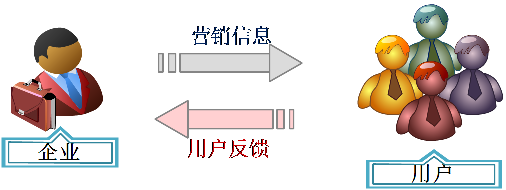
\includegraphics[width=0.5\textwidth]{直效营销示意图}
	\caption{直复营销场景示意图}
	\label{fig:直复营销示意图}
	\end{figure}

近年来,越来越多的机器学习技术被运用到直复营销领域中。最开始,研究人员通过使用监督学习中的经典分类模型,以营销决策的低错误率为学习目标,来解决上述直复营销问题。但是,因为在营销场景中,对不同客户的错误分类所带来的代价是不同的,所以传统的分类算法有很大的局限性。基于这个问题,学者们后续提出了很多基于代价敏感(cost-sensitive)的分类方法,在这些方法中,不同样本的错误分类有着不同的代价,因而可以取得比传统分类算法更好的性能。

但是,以上这些监督学习方法只能最大化单次决策的收益,即前一个决策和后一个决策之间是独立的。而在像直复营销这类应用场景中,随着时间的推移需要不断做出决策,因此属于序贯决策问题。所以,在进行营销决策时,不仅需要考虑单个决策的成本和收益,还要考虑到随着时间的推移,该次的决策对后续决策结果可能产生的影响。比如:在某一次营销活动时,某个客户所产生的预期收益可能会大于营销成本(即利润为负),但是,这次的营销可能会让该客户在之后的营销中产生更大的收益。所以,在某些时刻,为了能让客户在以后的营销活动中能够产生更多的利润,营销人员可能要牺牲短期的利润,以达到最大化客户生命周期价值的目的。而这对于基于监督学习或者非监督学习的机器学习算法很难办到的,

强化学习(Reinforcement Learning, RL)是机器学习的重要组成部分,主要用于解决序贯决策问题。其主要学习过程如图$\ref{fig:强化学习过程}$所示:通过智能体(Agent)不断地与环境(Environment)进行交互,并从环境反馈的延迟回报中学习状态与行为之间的映射关系,以使得可以达到累积奖赏最大化。从以上交互过程中,可以发现:强化学习在学习过程中考虑到了延迟回报,并且只关心当前采取什么行为可以使整个任务序列达到累积奖赏最大化,所以,强化学习可以很好的解决直复营销场景中,序列决策点之间相互影响问题,进而达到最大化客户生命周期价值的目标,这也是本文选择使用强化学习技术解决直复营销决策问题的出发点。特别地,本文主要关注基于值函数的强化学习算法。
\begin{figure}[htbp]
\centering
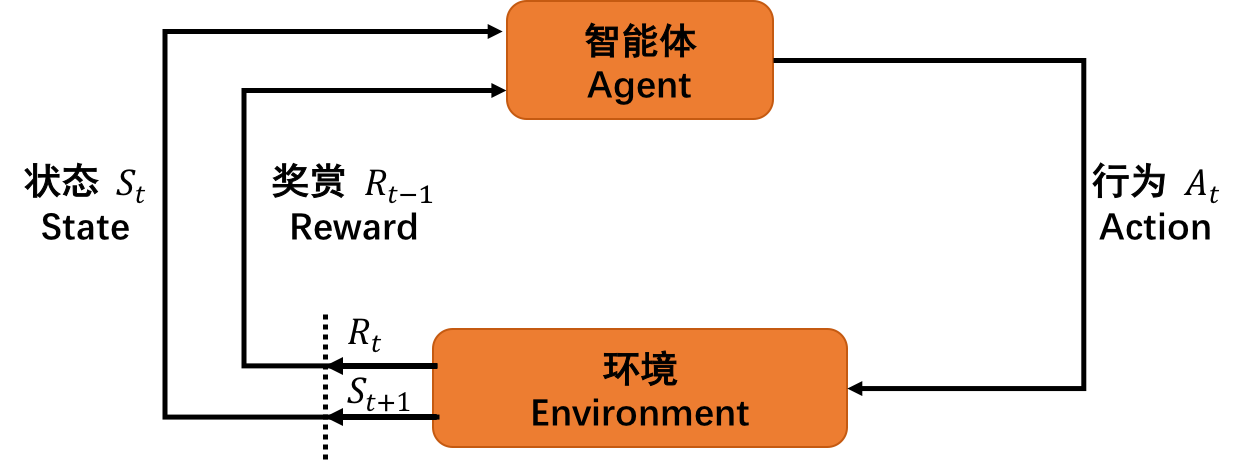
\includegraphics[width=0.8\textwidth]{强化学习过程_}
\caption{强化学习的交互过程}
\label{fig:强化学习过程}
\end{figure}

强化学习是从控制工程、心理学和运筹学等相关学科发展起来的。在上个世纪八十年代到九十年代,强化学习的理论基础研究取得了突破性进展,随后越来越多的被应用于工业控制、作业调度和机器学习等领域。比如,Macek等人将强化学习技术应用机器人躲避障碍物,Tesaruo等人结合神经网络将强化学习应用于西洋双陆棋中。近年来,DeepMind团队将深度强化学习技术结合蒙特卡罗树搜索,研发的AlphaGo大胜世界围棋冠军李世石和柯洁,从而在学术界和工业界再一次掀起了研究强化学习的高潮。

虽然强化学习的研究和应用已经取得了突破性的进展,但是由于强化学习问题本身的复杂性,加之不同应用场景的特殊性,强化学习在实际应用中任然面临一定的困难。在直复营销场景中,虽然近年来已经有学者开始使用强化学习技术来解决直复营销的决策问题,但是以下问题仍然没有得到有效的解决:

1)在不定期直复营销场景中,因为不同决策点之间的时间间隔是不固定的,会给奖赏信号带来一定的造成,影响值函数的学习和优化。

2)在实际应用中,随着数据量的提升,容易出现训练速度过慢、学习效率不高的问题。

3)在直复营销场景中存在客户状态的部分可观测问题,所以在实际应用中,为了更好地定义客户的状态以学习到最优策略,需要借助大量的专家领域知识。

本文针对以上三个问题进行分析,在基于值函数的强化学习方法中进行研究,并给出了相应问题的解决方案。

\section{研究现状}
本节首先对直复营销问题的研究现状进行介绍,主要包括三个方面:经典的分类算法、基于代价敏感的分类算法以及基于强化学习的方法。另外,因为本文主要是针对强化学习算法进行研究和改进的,所以之后也同样对强化学习的研究现状进行了介绍。

\subsection{直复营销的研究现状}
在机器学习领域,国内外关于直复营销策略的算法研究,可以概括为以下三个方面。

基于传统的经典分类算法。在文献\citep{alam2012actionable, ngai2009application, wong2005mining, coussement2015improving}中作者分别使用传统的逻辑回归算法、线性二次判别分析法、朴素贝叶斯、神经网络、决策树以及KNN等算法,对用户的响应模型进行建模,研究各类算法在直复营销中的应用效果,并从模型的可解释性和准确性方面给出了权衡建议。尽管这些算法在实际应用中取得了比使用人工经验营销决策好很多的效果,但是,这类算法在学习的时候假设误分类的代价是相同的,而在实际的直复营销应用中对不同客户误分类给企业所带来的损失是不同的,所以使用传统的分类算法必然会带来一定的局限性。

基于代价敏感的分类算法。针对以上传统经典分类算法在实际应用中存在的问题,众多学者又提出了基于代价敏感的分类算法。在文献\citep{bahnsen2015example}中,Bahnsen等将误分类代价加入到决策树的构建中,提出了最小代价决策树,并将其应用在了信用卡欺诈检测,信用评分和直接营销场景中,取得了比传统分类算法更好的效果。在文献\citep{cui2012cost}中,Cui等通过贝叶斯网络本身含有的先验概率计算出事例属于每个累的概率,然后使用经验风险公式直接对其进行代价敏感分类,用于解决直邮营销场景下的代价敏感的问题。这些基于代价敏感的分类算法虽然考虑到了误分类的不同代价问题,但是,在进行决策的时候每个决策点都是独立的,只能输出使的当前即时收益最大的策略,因此无法无法捕捉到直复营销序列决策中的相互影响,进而也达不到长期收益最大化目标。有关代价敏感算法的应用研究还有\citep{migueis2017predicting,zakaryazad2016profit,hu2015cost}

基于强化学习的算法。因为强化学习算法在学习过程中考虑到了决策序列之间的延迟影响,并且以最大化长期奖赏作为学习的目标,因此可以很好地解决直复营销场景中不同营销时刻之间的相互影响问题,进而达到最大化客户生命周期价值的目的。近年来,已经开始有学者尝试使用强化学习技术来解决营销中的相关应用问题。为了解决监督学习中独立决策的问题,Pednault等人\citep{pednault2002sequential}首次将强化学习技术用于解决直复营销问题中,提出了使用批强化学习解决该问题的框架,并且对仿真试验和评估方法提供了相应的解决方案。但是,对直复营销场景中的一些特殊问题并没有进行分析和讨论。Kim等人\citep{kim2009new}针对直复营销场景中的存在的客户流失问题,提出将客户的流失概率作为约束条件引入强化学习算法中,并试图在给定的阈值的情况下对其进行自动控制,试验证明该方法取得了比传统强化学习算法更好的营销策略。Boutilier等人\citep{boutilier2016budget}针对营销过程中存在的预算约束问题,引入带有预算约束的马尔科夫决策过程(Budgeted Markov Decision Process, BMDP),通过权衡预算分配和期望收益之间的关系得到一个关于预算约束的函数,并证明该函数是一个非递减的凹函数,最后使用强化学习方法求出该问题的解,试验证明该方法可以很好的解决带有预算约束的策略决策问题。Silver等人\citep{silver2013concurrent}提出了一种基于时间差分学习的并行强化学习框架。通过该框架可以并发的实现企业与客户之间的交互,并且通过模拟器分别在非自举(Non-bootstrappig)、非在线(Non-online)和非序列化(Non-sequential)三个方面进行了模型的对比评估,得到了在高并发的序列化问题中,应该考虑使用进行自举、在线学习以及使用序列化的强化学习方法的结论。但是,以上这些算法都没有考虑到在直复营销过程中的存在可变时间间隔问题,也没有很好的解决传统强化学习方法在实际应用中学习效率不高的问题。在深度强化学习方面。Tkachenko等人\citep{tkachenko2015autonomous}提出使用了深度强化学习解决直效营销中的问题,即使用Q-learning的方法训练一个深度神经网络来学习客户的状态和营销行为之间的关系,同时,该文章使用Recency-Frequency-Monetary(最近交易时间、交易频率和交易金额)指标参数化客户状态空间,实现了顾客响应率和顾客花费金额两方面的显著提高,但是该文章仅仅使用深度强化学习解决线性逼近方法表征能力不足的问题,而没有对神经网络在强化学习中的特征提取方法进行研究。

\subsection{强化学习的研究现状}

\paragraph{发展阶段}
强化学习的发展过程大概可以分为三个阶段。

第一阶段是1998年以前,这一阶段形成了强化学习基本理论框架,学者们关注最多是基于表格型的强化学习算法。代表性的工作是强化学习鼻祖Richard将其专刊装订成书\footnote{http://incompleteideas.net/book/bookdraft2017nov5.pdf},标志着强化学习发展成为机器学习领域的一个重要分支。
% 该书《Reinforcement Learning: An introdcution》是强化学习领域的经典著作,第一次系统而全面的介绍了强化学习的相关理论知识,至今仍然被广大的教育机构和强化学习爱好者作为强化学习的经典教材(该书最新电子版可在网上免费获取),
需要注意的是,这期间还出现了强化学习代表性算法Q-learning\citep{watkins1992q}和Sarsa\citep{rummery1994line}。

第二阶段是1998年到2013年,这一阶段基于直接策略搜索的强化学习方法得到了深入研究和发展。自从Williams在其论文\citep{williams1992simple}中提出直接对Reinforce算法的策略梯度进行估计这一方法后,出现了各种改进方法,如:GPOMDP\citep{baxter2001infinite}、PEGASUS\citep{neumann2005reinforcement}以及与值函数结合的Actor-Critic算法\citep{konda2000actor}等。

第三阶段是2013年以后,随着深度学习的发展,这一阶段出现了深度强化学习算法。代表性的工作是DeepMind团队提出了DQN(Deep Q Network)算法并将其成功应用在雅达利(Atari)游戏中\citep{mnih2013playing}。
其中,最具轰动性的事件当属在2016年和2017年,谷歌的AlphaGo利用深度强化学习算法连续两年分别击败了世界围棋冠军李世石和柯洁。
\paragraph{研究热点}

% 但是,目前强化学习在实际应用中仍然存在维度灾、收敛速度慢、时间信度分配等问题,其中维度灾是指在大空间和连续问题中,强化学习无法在有限的空间和时间内学习到一个合理的解决方案,而收敛速度慢又与强维度灾有着密切的关联,所以解决维度灾问题对强化学习的应用起到了十分重要的作用。

近年来,众多研究者主要集中于函数逼近的方法的研究,而函数逼近方法又可以分为参数化函数逼近方法和非参数化函数逼近方法。

参数化函数逼近方法又可以分为线性函数逼近和非线性函数逼近两种方法。其中在线性函数逼近中,基函数的形式和参数个数需要提前制定,往往会限制函数的逼近能力。该方法最早是由Samuel在1967年提出,并将其应用于西洋跳棋的系统设计中\citep{samuel1959some}。1988年,Sutton提出将线性函数逼近法与带有资格迹的时间差分(Temporal Difference, TD)方法相结合,然后使用梯度下降求解近似值函数的方法后\citep{sutton1988learning},掀起了线性函数逼近法研究的热潮,相继出现了最小二乘时间差分(Least Squares Temporal Difference, LSTD)算法\citep{bradtke1996linear}、离策略(Off-policy)函数逼近方法\citep{precup2001off}、以及梯度时间差分(Gradient Temporal Difference, GTD)学习算法\citep{sutton2009convergent}等,其中GTD解决了离策略TD学习算法的不稳定问题,且具有较低的时间复杂度\citep{sutton2009convergent}。

非线性函数逼近方法中的函数逼近器是关于参数的非线性函数,如神经网络。虽然该方法具有很强的表征能力,但是容易陷入局部最优,且收敛性难以保证。1995年Bertsekas等\citep{bertsekas1995neuro}利用前向神经网络逼近强化学习中的值函数,取得了相比线性逼近较好的结果,但是往往会出现不稳定不收敛的情况。直到DeepMind团队于2013年提出了DQN网络,才使的这一问题得到有效解决。在DQN网络中,通过在训练过程进行经验回放\citep{mnih2013playing}和单独设立目标网络\citep{mnih2015human}这两种改进方法,打破了数据之间的关联性,使的神经网络的训练过程收敛且稳定,并且在游戏中取得了令人振奋的表现。从此以后,彻底掀起了学术界和工业界研究深度强化学习的热情。2015年DeepMind团队又提出了Double DQN模型,在该模型中为了克服Q-learning本身固有的缺点——过估计(Overestimate),将动作的选择和动作的评估分别使用不同的值函数来实现。除此以外,深度Sarsa、A3C(Asynchronous Advantage Actor-Critic)、DDPG(Deep Deterministic Policy Gradient)等一些列有影响力深度强化学习模型相继被提出。

非参数化函数逼近法,并不是没有任何参数的函数逼近,而是指参数个数和基函数的形式并非固定,完全由样本决定,因此具有更大的灵活性和表征能力,但是当样本量很大时,将会带来更大的计算开销。非参数化函数逼近模型主要有基于高斯过程和基于核方法的值函数逼近模型。其中,基于核方法的研究相对较多,如基于核的强化学习函数逼近方法\citep{ormoneit2002kernel}、基于核的最小二乘TD方法(Kernel-based Least Squares TD, KLSTD)\citep{xu2005kernel}、基于最小二乘的策略迭代算法等(Kenel-based Least Squares Policy Iteration, KLSPI)\citep{xu2007kernel}等。

\paragraph{发展趋势}
强化学习正在飞速发展,从当前的研究工作中可以判断强化学习的发展具有如下趋势:1)强化学习与深度学习的结合会更加紧密。2)强化学习与领域知识的结合更加紧密,特别是在重塑回报函数的方向上。3)强化学习的理论分析会更加全面、具体,算法性能会更加稳定和高效。本文的研究工作正是从前两个方面展开的。

\section{主要研究内容}
强化学习在序贯决策的过程中,考虑到了序列中决策点之间的相互影响,并且以累积奖赏最大作为学习和优化目标,因此可以很好的解决传统的经典分类算法和基于代价敏感的分类算法在解决直复营销策略时决策独立性的问题。基于以上原因,本文选择使用强化学习的方法来研究直复营销策略,并针对直复营销场景中存在的营销决策点间的可变时间间隔问题、数据规模大学习效率不高问题以及客户状态的部分可观测问题,给出了相应的解决方法。如图$\ref{fig:研究路线图}$所示,本文的研究内容具体可以概括为以下四个方面:
\begin{figure}[htbp]
\centering
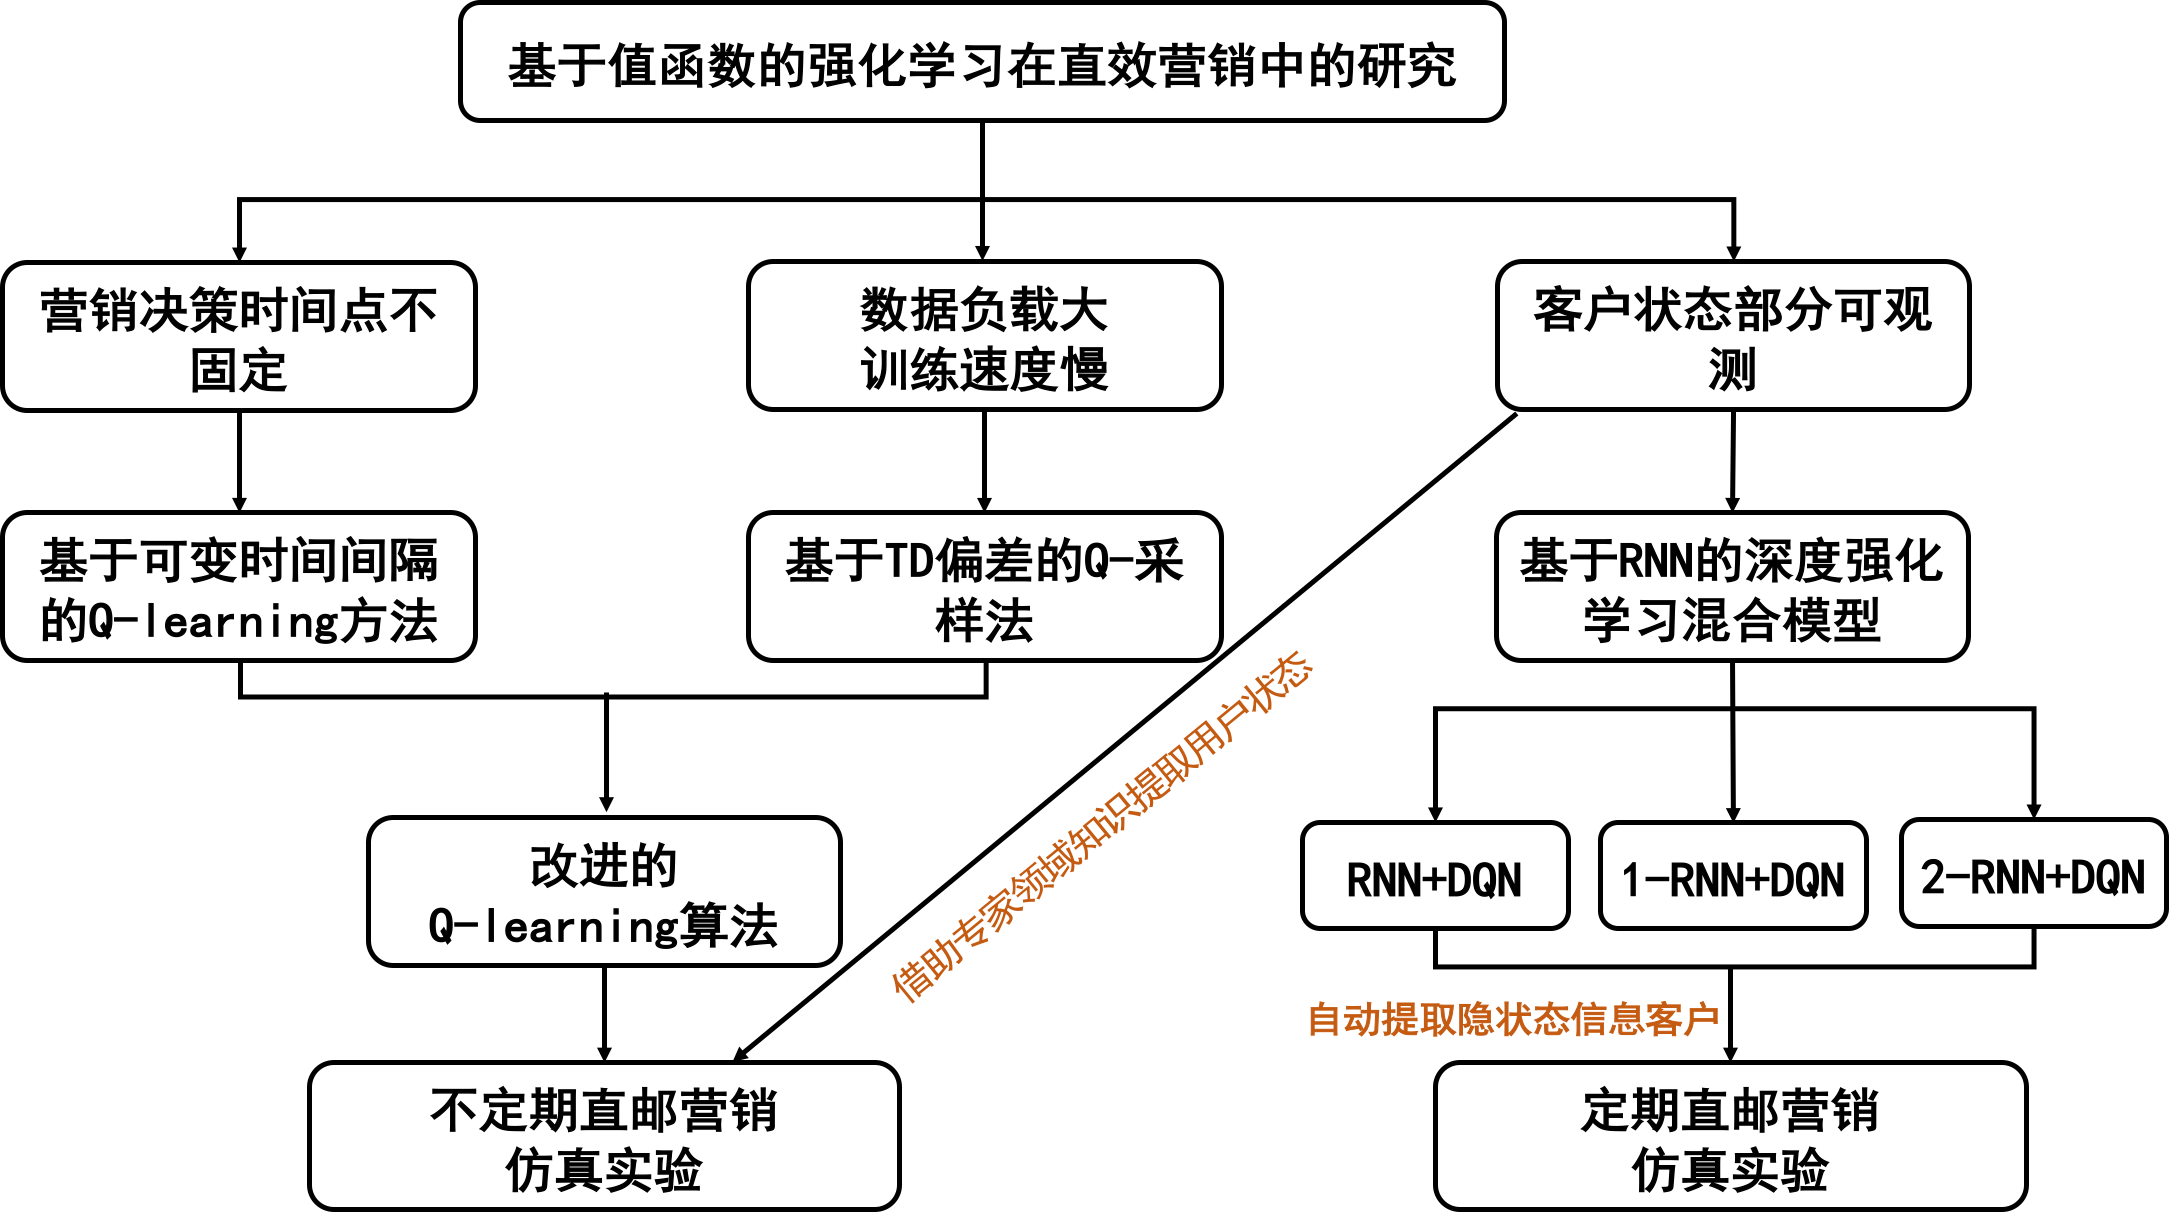
\includegraphics[width=1.0\textwidth]{研究路线图}
\caption{本文研究路线图}
\label{fig:研究路线图}
\end{figure}

1)基于经典的强化学习算法Q-learning进行研究,结合直复营销场景中决策点间可变时间间隔问题以及数据规模大学习效率不高的问题,提出了改进的Q-learning算法。具体地,首先,为了减少不同决策点之间的可变时间间隔给强化学习中的奖赏信号带来的噪声影响,提出使用均值归一化的方法进行解决。接着,针对Q值函数在迭代更新过程中因为时间间隔更新不同步问题而带来的偏差影响,提出一个标准化因子,并仿照值函数更新方法进行标准化因子的更新,从而可以有效的解决以上偏差问题。最后,为了解决在直复营销场景中,随着数据量的提升,Q-learning算法更新速度慢,学习效率不高的问题,在Q-采样的基础上,引入TD偏差,提出基于TD偏差的Q-采样方法,以减少训练次数的同时提高学习效果。

2)利用公开数据集进行模型的训练和仿真环境的构建,并针对1)中的两个改进点使用仿真环境进行模型的评估。其中,对于本文提出的基于可变时间间隔的Q-learning算法,从策略的长期收益和策略行为的变化情况两个角度进行模型的评估,通过试验表明本文所提的算法因为考虑到了可变时间间隔问题,在不定期直复营销场景中,相比传统的Q-learning算法,取得了更高的收益,并且策略的变化情况也更合理。另外,将本文所提的改进Q-采样方法从长期收益和采样数两个方面与Q-采样法和随机采样法进行比较,验证了所提算法在减少采样样本的同时可以取得更高的收益。需要说明的是,在以上两个实验中,为了解决客户状态的部分可观测问题,进而更好进行值函数的学习,引入了大量的专家领域知识来提取客户状态。

3)基于深度强化学习DQN模型进行研究,针对传统强化学习Q-learning在处理直复营销场景中的客户状态的部分可观测问题时,需要引入大量专家领域知识的问题,提出了基于RNN的深度强化学习混合模型。具体地,首先,结合直复营销场景的时序特点,提出使用基于RNN的DQN模型(DQN_RNN)来解决直复营销的决策问题。然后,指出DQN_RNN模型在网络优化过程中不能很好的同时处理隐状态的学习和值函数的逼近,并由此提出基于两个网络的混合模型:通过RNN网络从监督数据中学习到隐状态的表示方法后,再将隐状态作为DQN网络的状态输入进行强化学习,通过这种方式可以使的两个网络优势互补,在达到值函数逼近效果的同时也跟好地学习到了隐状态的表示方法,从而摆脱了需要借助专家领域知识的困扰。最后,为了达到更好的策略学习目的,又根据网络结构和参数训练方式的不同提出了三个改进模型:双网络独立训练模型、一步联合训练混合模型和两步联合训练混合模型。

4)利用公开数据集进行模型的训练和仿真环境的构建,并针对3)中的改进模型使用仿真环境进行模型的评估。首先从模型的长期收益上对所提算法进行评估,证明本文所提的深度强化学习混合模型相比基本的深度强化学习模型有更好的策略效果。然后,以随机的行为选择方式,利用仿真环境重新生成数据集对模型进行训练,试验结果表明数据收集时充分的探索对强化学习的学习效果至关重要。最后,使用不同的规模的数据集对模型进行训练,试验结果表明所提模型不需要利用大批量数据进行训练同样可以产生较好的营销策略。

\section{论文的结构安排}
基于传统的监督学习和非监督学习方法在序贯决策问题上的局限性,本文考虑使用强化学习的方法来解决直复营销中的决策问题,以使的最大化客户的生命周期价值,进而达到最大化企业长期收益的目的。针对直效营销场景中的营销决策点时间不固定和数据负载大使用效率不高的问题,在传统的Q-learning算法的基础上提出了相应的改进意见。另外,针对在实际应用中,传统的强化学习方法不能很好的处理客户的部分可观测问题,使用深度强化学习的方法以学习隐状态的方式进行解决,进一步地,为了更好的学习隐状态的表征能力,进而提高值函数的逼近效果,又提出了基于RNN的深度强化学习混合模型。本文共分为五章,具体每章的研究内容如下:

第一章: 绪论 \quad 本章首先对直复营销的场景、目的以及研究意义进行介绍,指出传统的监督学习和非监督学习在处理该问题时的不足,由此引出了强化学习的方法,并对强化学习进行简单阐述。接着,分别接着直复营销以及强化学习的国内外研究现状,并结合本文的研究内容进行分析。最后,概括论述了本文的主要研究内容,并对论文的结构安排进行了说明。

第二章: 相关理论概述 \quad 本章首先对强化学习方法的过程进行总体阐述,以便让读者对强化学习方法有一个总体的认识。接着,对强化学习的理论框架马尔科夫决策过程以及强化学习的三个基本要素(策略、回报和值函数)进行介绍。然后,针对基于值函数的三个经典的强化学习方法进行讲解,以便让读者更好的理解强化学习的思想和求解方法。最后,对值函数的逼近方法进行讨论,阐述各自的优缺点以及适应场景,特别地,对非线性函数逼近方法中的DQN模型进行了详细阐述,为后续章节打下理论基础。

第三章: 基于改进的Q-learning算法在直复营销中的研究 \quad 本章首先介绍研究动机,即为什么使用强化学习的方法进行直复营销策略的研究。接着,将传统的经典强化学习算法Q-learning应用于直复营销的策略决策上,并针对现实应用中存在的营销决策点间的可变时间间隔问题和数据负载大学习效率低的问题,提出对应的解决方法。最后,利用不定期直邮营销的数据集构建仿真环境,对所提模型和对照模型进行评估,并对评估结果进行分析。最后

第四章: 基于深度强化学习混合模型在直复营销中的研究 \quad 本章首先介绍研究动机,即为什么使用深度强化学习的方法来解决直复营销中的决策问题。接着,介绍DQN模型以及基于RNN的DQN模型(DQN_RNN),然后分析DQN_RNN在优化学习过程中的不足,提出了基于两个网络的混合模型,并针对网络结构和训练方法进行分析,提出了一系列改进的方法,主要包括:双网络独立训练模型、一步联合训练混合模型和两步联合训练混合模型。最后,在定期直邮营销数据集中构建仿真环境,从不同角度来评估模型的试验结果,并对试验结果进行分析和总结。

第五章: 总结与展望 \quad 本章系统的总结了本文的工作内容,并指出了本文工作存在的不足以及下一步的研究和工作方向。



